\documentclass[11pt,a4paper]{article}

\usepackage{fontspec}
\usepackage{geometry}
\usepackage{graphicx}
\usepackage{xcolor}
\usepackage{multicol}
\usepackage{enumitem}
\usepackage{fancyhdr}

\geometry{top=11mm,bottom=12mm,left=14mm,right=14mm}
\setlength{\parindent}{0pt}
\setlength{\parskip}{1.8pt}
\setlength{\columnsep}{6mm}
\setlength{\multicolsep}{3pt plus 1pt minus 1pt}
\setlength{\footskip}{7mm}
\raggedcolumns
\sloppy

\defaultfontfeatures{Ligatures=TeX}
\setmainfont[
  Path=../../node_modules/@expo-google-fonts/readex-pro/,
  UprightFont=400Regular/ReadexPro_400Regular.ttf,
  BoldFont=700Bold/ReadexPro_700Bold.ttf
]{Readex Pro}
\newfontfamily\displayfont[
  Path=../../node_modules/@expo-google-fonts/alexandria/,
  UprightFont=700Bold/Alexandria_700Bold.ttf,
  BoldFont=800ExtraBold/Alexandria_800ExtraBold.ttf
]{Alexandria}

\definecolor{Ghaf}{HTML}{1D684F}
\definecolor{Forest}{HTML}{12372D}
\definecolor{Mangrove}{HTML}{28736C}
\definecolor{DateGold}{HTML}{B87524}
\definecolor{Ivory}{HTML}{F3F0E7}
\definecolor{LeafMist}{HTML}{EDF1E8}
\definecolor{Ink}{HTML}{172621}
\definecolor{Muted}{HTML}{606B65}
\definecolor{Line}{HTML}{CBCDC2}

\color{Ink}
\pagestyle{fancy}
\fancyhf{}
\renewcommand{\headrulewidth}{0pt}
\fancyfoot[L]{\fontsize{8}{9}\selectfont\color{Muted}Ghaf competition brief}
\fancyfoot[R]{\fontsize{8}{9}\selectfont\color{Ghaf}\thepage\ / 2}

\newcommand{\briefsection}[2]{%
  \vspace{1.5pt}%
  {\displayfont\fontsize{10.8}{12.4}\selectfont\color{Ghaf}#1. #2}\par
  \vspace{0.3pt}%
}

\newcommand{\briefheading}[1]{%
  \vspace{1.5pt}%
  {\displayfont\fontsize{10.8}{12.4}\selectfont\color{Ghaf}#1}\par
  \vspace{0.3pt}%
}

\newcommand{\smallcaption}[1]{%
  {\fontsize{7.8}{9.2}\selectfont\color{Muted}#1}%
}

\begin{document}
\thispagestyle{fancy}

\noindent
\begin{minipage}[c]{0.11\textwidth}
  
\includegraphics[width=\linewidth]{assets/ghaf-mark.png}
\end{minipage}\hfill
\begin{minipage}[c]{0.86\textwidth}
  {\fontsize{8.4}{9.6}\selectfont\color{Mangrove}\textbf{KHALIFA UNIVERSITY SMAC 2026}\hfill WORKING COMPETITION PROTOTYPE}\par
  \vspace{1.2mm}
  {\displayfont\fontsize{23}{25}\selectfont\color{Forest}GHAF: SMALL FAMILY ACTIONS,\\VISIBLE GROWTH}\par
  \vspace{0.8mm}
  {\fontsize{11.2}{13.4}\selectfont\color{Muted}An Arabic-first mobile app that turns safe daily responsibilities into family recognition and a shared UAE garden.}
\end{minipage}

\vspace{2.2mm}
\noindent
\includegraphics[trim=0 255 0 255,clip,width=\textwidth]{assets/ghaf-habitat.jpg}
\vspace{0.4mm}

\smallcaption{The Ghaf landscape gives one clear memory of the product: useful actions grow into a shared family story.}

\vspace{1.2mm}
\begin{multicols}{2}

\briefsection{1}{Executive Overview}
Ghaf is a working mobile prototype for UAE families with children aged 6 to 14. A Parent approves a clear responsibility, a Child chooses and completes it with allowed help, and the Parent confirms the result. Eligible work earns fixed symbolic Seeds that grow a private garden based on UAE landscapes. This matters because family tasks are often discussed only after something is missed. Ghaf provides a calmer path built around choice, support and specific praise. The competition journey runs offline with synthetic family data.

\briefsection{2}{Problem and Opportunity}
Many routine apps depend on reminders, points or public comparison. This can place the Parent in a policing role and give the Child little support when a task is unclear, too large or unsafe. Environmental learning can also feel distant from home life. Ghaf uses an ordinary task as a small, visible learning moment. A clearer agreement around the task helps the family recognise useful effort without shame or loss.

\briefsection{3}{Proposed Solution}
Ghaf keeps Parent and Child experiences separate inside one Expo application. The Parent selects from eight reviewed task categories, checks safety and privacy, and approves the exact definition of done. The Child sees approved choices, short steps and ways to ask for help, retry or request a smaller equivalent. Once the Parent confirms, the system records praise and applies the fixed result only once. Seeds never decrease and the garden never withers after a missed day. Five UAE landscape tracks make progress easy to understand. In the main demo, a supervised recycling task awards 12 Seeds, grows the Mangrove track and adds one privacy-filtered family contribution.

\briefsection{4}{Target Users and Use Case}
The main users are Parents or guardians and children who share daily responsibilities. Salem, a synthetic nine-year-old profile, receives the Green Impact task. His Parent checks its safety notes and uses the prepared Ghaf Guide to simplify the wording. In the separate Child space, Salem reads the steps and asks an adult to check the materials and manage the route to the bin. Submission alone gives no reward. His Parent reviews the task, gives action-specific praise and confirms it. Salem then receives the displayed 12 Seeds and sees the Mangrove garden grow.

\briefsection{5}{Innovation and Competitive Advantage}
Ghaf's main difference is its complete decision chain. Assistant content cannot assign a task, judge the Child or issue a reward. The default examples are prepared, clearly labelled and limited to the approved task. Privacy rules run before a shared counter or image changes. In the private weekly League, each Child has five equal Challenge Leaves, scores stop at 100, ties share a place, and permitted help keeps full credit. The family view grows one combined canopy rather than comparing raw Seed totals. Family Rewards remain private Parent promises, not payments. This creates a fair, locally relevant experience while keeping the demonstration reliable offline.

\end{multicols}

\newpage
\thispagestyle{fancy}

{\displayfont\fontsize{14.5}{16}\selectfont\color{Forest}PAGE 2 - FUNCTIONALITY AND TECHNICAL IMPLEMENTATION}\par
\vspace{0.8mm}

\noindent
\begin{minipage}[t]{0.29\textwidth}
  \centering
  
\includegraphics[height=3.35cm]{assets/parent-dashboard.png}\par
  \smallcaption{Parent dashboard: task and family canopy}
\end{minipage}\hfill
\begin{minipage}[t]{0.29\textwidth}
  \centering
  
\includegraphics[height=3.35cm]{assets/child-task.png}\par
  \smallcaption{Child view: one approved task and clear help}
\end{minipage}\hfill
\begin{minipage}[t]{0.29\textwidth}
  \centering
  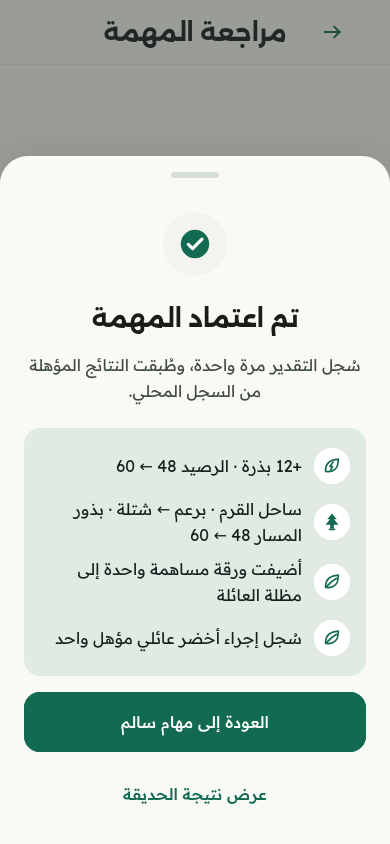
\includegraphics[height=3.35cm]{assets/approval-result.png}\par
  \smallcaption{Parent approval: one complete, fixed result}
\end{minipage}\par

\vspace{0.2mm}
\begin{multicols}{2}

\briefsection{6}{Core Functionality}
\begin{enumerate}[leftmargin=*,label=\textbf{\arabic*.},itemsep=0.8pt,topsep=0.5pt]
  \item \textbf{Separate access.} Parents use local verification. Children use a PIN, picture sequence or approved pairing. A remembered device stores one checked marker, not a password.
  \item \textbf{Task building.} The Parent selects a reviewed template. Ghaf shows supervision, privacy, fixed Seeds and landscape before approval.
  \item \textbf{Child action.} The Child starts the task, reads its finish condition, requests bounded help and submits.
  \item \textbf{Parent check-in.} The Parent confirms, requests a kind retry or accepts an agreed equivalent. Repeated confirmation gives no second reward.
  \item \textbf{Growth views.} Confirmation updates eligible Seeds, landscape and family progress through separate rules.
\end{enumerate}

\briefsection{7}{User Journey}
Ghaf opens in Arabic RTL and can change to English LTR. A Parent signs in, restores the synthetic family and approves a task. After sign-out, the Child enters the separate space, uses support if needed and submits. The Parent returns, reviews the work and gives praise. One final action commits the result. The Garden changes permanently, while shared views receive only permitted information. A Parent-only reset restores the Arabic starting state.

\briefsection{8}{Technical Design}
The frontend is one Expo 57 and React Native 0.86 app written in strict TypeScript 6. Expo Router separates Parent and Child routes. Zustand manages the resettable session, while policy modules own task, Garden, League, reward and assistant rules. i18next supplies Arabic and English copy with logical RTL and LTR layouts.

There is no production database or account backend. Native builds use Expo SQLite key-value storage for the local family directory and device marker; web preview uses localStorage. Versioned records fail closed when invalid. Deterministic services run by default. Reference Cloudflare Workers exist for bounded AI experiments, but the flags are off and no deployment is claimed. Remote adapters use typed schemas, timeouts and safe fallbacks, with no provider secret in the mobile app.

\briefsection{9}{Feasibility, Scalability and Reliability}
Packaged data, offline fallback, route guards and one-time confirmation make the judge journey repeatable. Automated tests cover access, privacy, rewards, localisation and reset. Service interfaces allow reviewed remote systems to replace local providers later. The present scale is one synthetic household. Physical Android accessibility and human review remain acceptance work, so Ghaf is presented as a prototype.

\briefsection{10}{Impact and Future Development}
Ghaf can turn repeated reminders into a clear family agreement about the task, allowed help and observed result. The Child keeps choice and sees how an action supports a family goal. Reviewed activities include recycling, water care and switching off unused lights. The garden is symbolic and does not claim measured environmental impact.

Next steps are physical Android review in both languages, accessibility tests and named cultural, safeguarding and image-rights approval. Production use also needs secure identity, consent, recovery and a reviewed server boundary before real Child data or live AI. Ghaf merits recognition because its central idea works now: a safe family action becomes specific human praise and lasting shared growth.

\end{multicols}

\end{document}
